\documentclass{article}
\usepackage[margin={1.5cm,1.5cm}]{geometry}

\usepackage{listings}
\usepackage{color}
\usepackage{tabularx}
\usepackage{pdfrender}
\usepackage{amssymb}
\usepackage{bussproofs}
\usepackage{graphicx}
\usepackage{multicol}
\usepackage{amsmath}
\usepackage{hyperref}

\definecolor{mygreen}{rgb}{0,0.6,0}
\definecolor{mygray}{rgb}{0.5,0.5,0.5}
\definecolor{mymauve}{rgb}{0.58,0,0.82}

\def \extends{$<:$}
\setlength{\columnsep}{1cm}

\lstset{ 
  backgroundcolor=\color{white},  
  basicstyle=\footnotesize,     
  breakatwhitespace=false, 
  breaklines=true,       
  captionpos=b,   
  commentstyle=\color{mygreen},  
  frame=single,	     
  keepspaces=true,
  keywordstyle=\color{blue},      
  language=Octave,                 
  numbersep=5pt,               
  showspaces=false,                % show spaces everywhere adding particular underscores; it overrides 'showstringspaces'
  showstringspaces=false,          % underline spaces within strings only
  showtabs=false,                  % show tabs within strings adding particular underscores
  stepnumber=2,                    % the step between two line-numbers. If it's 1, each line will be numbered
  stringstyle=\color{mymauve},     % string literal style
  tabsize=2,	                   % sets default tabsize to 2 spaces
  title=\lstname                   % show the filename of files included with \lstinputlisting; also try caption instead of title
}

\title{Mid-term paper for Programming Theory class}
\author{Ogiwara}
\date{\today}
\begin{document}
\begin{multicols}{2}
[
\maketitle
]
\section{Objective}
Pick one programming language, and explain about that.
At here, I'll explain about Pony language \cite{ponylang} through description of features and performance, sample codes, and reference capability type system, which is the key concept of this language.

\subsection{Why I chose Pony}
This is really boring reason. I just seek "200 minor programming language list"\cite{200}, and I found this.  

\section{Features and Performance}

\subsection{Simple introduction from official page \cite{ponylang}}
Pony is an open-source, object-oriented, actor-model, capabilities-secure, high-performance programming language. 

Type safe. Really type safe. On top page, there is a link for mathematical proof paper \cite{type-proof-paper}. I will explain about that in later section.

Memory safe. There are no dangling pointers and no buffer overruns. The language doesn't even have the concept of \texttt{null}. 

Exception-Safe. There are no runtime exceptions. All exceptions have defined semantics, and they are always caught. 

Data-race Free. Pony doesn’t have locks nor atomic operations or anything like that. Instead, the type system ensures at compile time that your concurrent program can never have data races. So you can write highly concurrent code and never get it wrong. 

Deadlock-Free. This one is easy because Pony has no locks at all. So they definitely don’t deadlock, because they don’t exist.

\subsection{Example Code}

\lstinputlisting{timer.pony}

Here is timer program in Pony.
At first sleeps for 5 seconds, and after that, repeat to run Notify.apply method in every 2 seconds.

There are \texttt{Main} actor and \texttt{Notify} class. 
\texttt{Main} actor has \texttt{new create} symbol, which works as constructor.
\texttt{Notify} class has \texttt{ \_env}, \texttt{ \_counter} fields, \texttt{create} constructor, and \texttt{apply} method.

First, \texttt{Main} actor ' \texttt{create} constructor is called. It is initial function as same as \texttt{int main()} in C or \texttt{public static void main(String[] args)} in Java. 

Values are assigned into \texttt{timers} and \texttt{timer}, and then \texttt{Timers.apply} method is called. 
At here, \texttt{Timers} is another actor, so we have to move \texttt{timer} data to the actor by \texttt{consume} expression.

 \texttt{Timers} actor calls passed object(At here \texttt{Notify})'s apply method repeatedly (At here sleeps for 5 seconds run every 2 seconds). 
 
\texttt{Notify.apply} outputs current \texttt{\_counter}, and then increment it.




\subsection{Compare to other languages}

\begin{lstlisting}[language=Erlang]{Make actor in Elixir}
defmodule Actor1 do
	def call() do
		...
	end	
end	

GenServer.start_link(Actor1, [:call])
\end{lstlisting}

To use actor, Elixir\cite{elixir} have to define module, and make actor by specifying both module name and method name.

\begin{lstlisting}{Make actor in Pony}
actor Actor1
	be call() =>
		...
		
let actor1 = Actor1		
\end{lstlisting}

However in Pony, \texttt{actor} is primitive syntax, so you can just make instance of actor as same as classes. \\





\begin{lstlisting}{ownership system in Rust}
let a = String::new("hello")
let b = a
// You can't use a at here anymore.
\end{lstlisting}

\begin{lstlisting}{consuming in Pony}
let a : String iso = "hello"
let b = consume a
// You can't use a at here anymore.
\end{lstlisting}

Pony has much more stronger reference capability type system than Rust \cite{rust} 's ownership type system. 

At here, \texttt{iso} is one of reference capability types, which mean "this value is readable in writable in one actor, and it can move to another actor".

About reference capability, I will explain about it in later section.
\\



\begin{lstlisting}[language=Python]{Python indentation}
class A:
	def b():
		...
\end{lstlisting}

\begin{lstlisting}{Pony indentation}
class A
	fun b() =>
		...
\end{lstlisting}


Pony uses indentation as block as same as Python\cite{python}.\\

\begin{lstlisting}[language=Ruby]{do end block style both in Ruby and Pony }
for i in values do
	
end		
\end{lstlisting}

 Pony uses do$\sim$end style block as same as Ruby \cite{ruby}. \\


\begin{lstlisting}[language=Java]{Type parameter and apply method in Scala}
class A[T]{
	def apply(i: T){}
}	

val a: A[Int] = new A()
a(8)
\end{lstlisting}

\begin{lstlisting}{Generics and apply method in Pony}
class A[T]
	fun apply(i: T) =>
		...
	
let a: A[Integer] = A
a(8)	
\end{lstlisting}

Pony uses square brackets([T]) for Generics, and functional style \texttt{apply} method as same as Scala\cite{scala}. \\


\begin{lstlisting}{interface in Go}
type geometry interface {
    area() float64
    perim() float64
}

type rect struct {
    width, height float64
}

func (r rect) area() float64 {
    return r.width * r.height
}
func (r rect) perim() float64 {
    return 2*r.width + 2*r.height
}
// Now type rect implements geometry interface.

\end{lstlisting}

\begin{lstlisting}{interface in Pony}
interface Animal
	fun bark(): String
	
class Dog
	fun bark(): String
		=> "Bow!"	
	
// Now type Dog implements Animal interface.
// You can annotate Dog implements Animal by 
// class Dog is Animal
\end{lstlisting}
 
Pony has structural subtyping as same as Go\cite{go}.


\begin{table*}[]
\centering
\begin{tabular}{lllll}
\hline
                          & Pony & Scala & Elixir & Rust \\ \hline \hline
Zero-Copy                 & $\checkmark$ & $\checkmark$& &  $\checkmark$    \\ \hline
Data-race free            & $\checkmark$ &       & $\checkmark$& $\checkmark$ \\ \hline
Statically data-race free & $\checkmark$ &       &        &      \\ \hline
Read unique (iso)         & $\checkmark$&       &        &      \\ \hline
Write unique (trn)        & $\checkmark$&       &        &      \\ \hline
Mutability (ref)          &$\checkmark$ &$\checkmark$ &        &$\checkmark$ \\ \hline
Immutability (val)        &$\checkmark$&       & $\checkmark$& $\checkmark$\\ \hline
Identity (tag)            &$\checkmark$&       &        &      \\ \hline
Actors                    &$\checkmark$& $\checkmark$ & $\checkmark$&      \\ \hline
Formal proof              &$\checkmark$&       &        &      \\ \hline
\end{tabular}
\caption{Feature comparison.\cite{type-proof-paper}}
\end{table*}

Table 1 is summary of some parallarel features of Pony and compare with Scala, Elixir, and Rust.

\subsection{Performance}


\begin{figure*}
\centering 		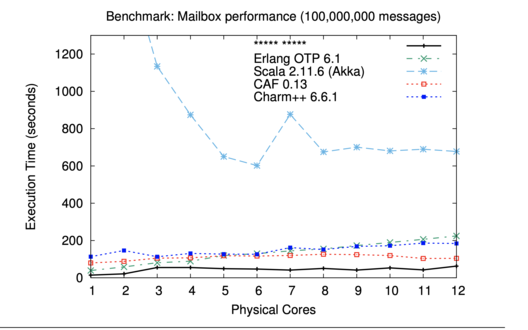
\includegraphics[width=0.6\textwidth]{a}
\caption{Actor creation, where **** is Pony. \cite{type-proof-paper}}
\end{figure*}



\begin{figure*}
\centering 		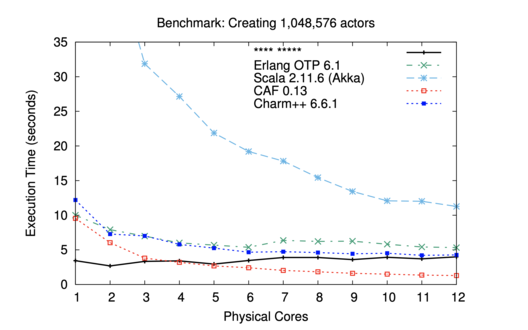
\includegraphics[width=0.6\textwidth]{b}
\caption{Mailbox performance, where **** is Pony. \cite{type-proof-paper}}
\end{figure*}


Figure 1 and Figure 2 is performance comparison graph with Erlang, Scala, CAF, Charm++, and Pony from the paper\cite{type-proof-paper}.
Figure 1 shows actor creation performance, and figure 2 shows mailbox performance.


\section{Reference capability type system}
Combining the actor-model with shared memory for performance is efficient but can introduce data-races. Well known approaches to static data-race freedom are based on uniqueness and immutability, but lack flexibility and high performance implementations. Pony's approach, based on deny properties allow reading, writing and traversing unique references, introduced a new form of write uniqueness, and guaranteed atomic behaviours.

\subsection{Deny properties}
Rather than indicate which operations are allowed on a reference, Pony's capabilities indicate what operations are denied on other references to the same object. It is distinguished what is denied to the actor that holds a reference(local aliases) from what is denied to all other actors(global aliases). Each capability stands for a pair of local and global deny properties.
These are shown in table 1\cite{type-proof-paper}, and we call it "Reference capability matrix". For example, \texttt{ref} denies global aliases that can read from or write to the object, but it allows local aliases to both read from and write to it.

No capability can deny local aliases that it allows globally.  Therefore, some cells in the matrix are empty.
These deny properties are used to derive the operations permitted on a reference, and determine the ability of each capability references. \\

\texttt{iso} is for references to isolated data structures. If you have an \texttt{iso} varibale then you know that there are no other variables that can access that data. So you can change it however you like and give it to another actor. 

\texttt{iso} is read and write unique, there can only be one reference at a time that can only be one reference at a time that can be used for reading or writing.

Because \texttt{iso} has read and write uniqueness, it can send the value to other actors(This is called \textit{Sendable}).\\

\texttt{val} is for references to immutable data structures. If you have a val variable then you know that no-one can change the data. So it is \textit{Sendable}, and you can read it and share it with other actors.\\


\texttt{ref}  is for references to mutable data structures that are not isolated, in other words, “normal” data. If you have a \texttt{ref} variable then you can read and write the data however you like and you can have multiple variables that can access the same data. But you can’t share it with other actors.\\

\texttt{box} is for references to data that is read-only to you. That data might be immutable and shared with other actors or there may be other variables using it in your actor that can change the data. Either way, the box variable can be used to safely read the data. This may sound a little pointless, but it allows you to write code that can work for both val and ref variables, as long as it doesn’t write to the object.\\

\texttt{trn} has write uniqueness, and is used for data structures that you want to write to, while also holding read-only (box) variables for them. You can also convert the \texttt{trn} variable to a \texttt{val} variable later if you wish, which stops anyone from changing the data and allows it be shared with other actors. \\

\texttt{tag} is for references used only for identification. You cannot read or write data using a tag variable. But you can store and compare tags to check object identity and share(Sendable) \texttt{tag} variables with other actors.

\subsection{Type system}
By including reference capabilities to its type system, Pony finds all the errors at compile time, and guarantees no runtime error.

\begin{figure*}
\centering
	
\AxiomC{T$<$:T''}
\AxiomC{T''$<$:T'}
\BinaryInfC{T $<$: T'}
\DisplayProof 

\proofSkipAmount

\AxiomC{}
\UnaryInfC{S $\kappa \circ <:$ S $\kappa$ }
\DisplayProof

\proofSkipAmount

\AxiomC{$\kappa <: \kappa'$}
\UnaryInfC{S $\kappa <:$ S $\kappa'$ }
\DisplayProof

\proofSkipAmount

\texttt{iso} \extends \texttt{trn} \extends \{\texttt{ref},\texttt{val}\} \extends \texttt{box} \extends \texttt{tag} 

\proofSkipAmount

\textit{Schedule}(T) \textit{iff} T = S $\kappa \land \kappa \in $ \{ \texttt{iso},\texttt{val},\texttt{tag} \}	

\proofSkipAmount
\caption{Sub-types and sendable types \cite{type-proof-paper}}
\end{figure*}

Subtyping relationship of reference capabilities are shown in fig 1. At here, $\kappa$ is reference capability, $\circ$ is temporary type, \extends is showing that left-side type is subtype of right-side type. 

When reading a field \texttt{f} ftom an object $\iota$ we obtain a temporary. The capability of this temporary must be a combination of $\kappa$, the capability of the path leading to $\iota$, and $\kappa'$, then capability with which $\iota$ sees the field. Pony express this through the operator $\triangleright$, defined in table 2.


Storing a reference into a field of an object $\iota$ is legal if the type of the reference is both a subtype of the type of the field and also safe to write into the origin. The relation $\kappa \triangleleft \kappa'$, as defined in table 3. \\


Through applying subtyping rule and viewpoint adaption to reference capability, type proof theory guarantees that well-formed heap ensures data race freedom, and it is preserved.

\newtheorem{theorem}{Theorem}
\begin{theorem}
	A well-formed heap ensures data race freedom.
	
	$\forall \Delta,\chi,\alpha_1,\alpha_2,\texttt{f,g},$ if
	
	\begin{enumerate}
		\item $\Delta \vdash \chi \Diamond,$ and
		\item $\chi(\alpha_1) = (\_,\_,\sigma_1, \_,  E_1[z_1.\texttt{f} = z_3])$, and
		\item $\chi(\alpha_2) = (\_,\_,\sigma_2, \_,  E_2[z_2.\texttt{g}])$
	\end{enumerate} 
	
	then $\chi(\alpha_1, |\sigma_1|\cdot z_1) \neq \chi(\alpha_2, |\sigma_2| \cdot z_2)$
\end{theorem}

\begin{theorem} 
	Well-formedness is preserved.
	
	$\forall \Delta, \chi, if \Delta \vdash \chi \Diamond and \chi \rightarrow \chi' then  \exists \Delta'.\Delta' \vdash \chi'\Diamond$
\end{theorem}

Proof of these theorems are written in paper \cite{type-proof-paper}.


\begin{table*}[]
\begin{tabularx}{\textwidth}{|X|X|X|X|}
 \hline
 & Deny global read/write aliases & Deny global write aliases & Allow all global aliases \\  \hline
Deny local read/write aliases & \textit{Isolated(iso) }    &                           &                        \\  \hline
Deny local write aliases      & Transition(\texttt{trn})                & \textit{Value(val)  }              &                        \\  \hline
Allow all local aliases       & Reference(\texttt{ref})                 & Box(\texttt{box})                  & \textit{Tag(tag)  }             \\  \hline
                              & (Mutable)                      & (Immutable)               & (Opaque)   \\ \hline           
\end{tabularx}
\caption{Capability matrix. Capabilities in \textit{italics} are sendable.\cite{type-proof-paper} }
\end{table*}

\begin{table*}[]
\centering
\begin{tabular}{lllllll}
\hline
$\kappa \triangleright \kappa'$ & \multicolumn{6}{c}{$\kappa'$}             \\ \hline
$\kappa$                 & iso & trn & ref & val & box & tag \\ \hline \hline
iso               & iso & tag & tag & val & tag & tag \\ \hline
trn               & iso & trn & box & val & box & tag \\ \hline
ref               & iso & trn & ref & val & box & tag \\ \hline
val               & val & val & val & val & val & tag \\ \hline
box               & tag & box & box & val & box & tag \\ \hline
tag               &  $\bot$ & $\bot$ & $\bot$ & $\bot$ & $\bot$ &     \\ \hline
\end{tabular}
\caption{Viewpoint adaption.\cite{type-proof-paper}}
\end{table*}


\begin{table*}[]
\centering
\begin{tabular}{lllllll}
\hline
$\kappa \triangleleft \kappa'$ & \multicolumn{6}{c}{$\kappa'$}             \\ \hline
$\kappa$                 & iso & trn & ref & val & box & tag \\ \hline \hline
iso               & $\checkmark$ &  &  & $\checkmark$ &  & $\checkmark$ \\ \hline
trn               & $\checkmark$ & $\checkmark$ &  & $\checkmark$ &  & $\checkmark$ \\ \hline
ref               & $\checkmark$ & $\checkmark$ & $\checkmark$ & $\checkmark$ & $\checkmark$ & $\checkmark$ \\ \hline
val               &  &  &  &  &  &  \\ \hline
box               &  &  &  &  &  &  \\ \hline
tag               &   &  &  &  &  &     \\ \hline
\end{tabular}
\caption{Safe to write.\cite{type-proof-paper}}
\end{table*}




\begin{thebibliography}{9}
\bibitem{ponylang}
Pony language official page
\\\texttt{https://www.ponylang.io}

\bibitem{type-proof-paper}
Deny Capabilities for Safe, Fast Actors
\\\texttt{https://www.ponylang.io/media/papers/fast-cheap-with-proof.pdf}

\bibitem{elixir}
Elixir language official page
\\\texttt{https://elixir-lang.org}

\bibitem{rust}
Rust language official page
\\\texttt{https://www.rust-lang.org}

\bibitem{python}
Python language official page
\\\texttt{https://www.python.org}

\bibitem{ruby}
Ruby language official page
\\\texttt{https://www.ruby-lang.org/en/}
	
\bibitem{scala}
Scala language official page
\\\texttt{https://www.scala-lang.org}

\bibitem{go}
Go language official page
\\\texttt{https://golang.org}
	

\bibitem{200}
200 minor programming language
\\\texttt{ \url{https://qiita.com/make_now_just/items/b2ab19f954417c71848d} }

\end{thebibliography}
\end{multicols}
\end{document}
